\documentclass[12pt, a4paper]{article}

\usepackage{polski}
\usepackage[utf8]{inputenc}
\usepackage{hyperref}
\usepackage{graphicx}
\usepackage{color}

\author{M.~Karpiuk}
\title{Projekt z \LaTeXe}
\date{05.12.2014}

\linespread{1.2}

\begin{document}


\maketitle


\newpage
\tableofcontents


\newpage
\section{Definicja}
\indent
Macierz odwrotna – element odwrotny w pierścieniu macierzy kwadratowych. Uogólnieniem pojęcia macierzy odwrotnej jest tzw. uogólniona macierz odwrotna.
\\\\
\indent
Niech $A$ będzie macierzą kwadratową ustalonego stopnia. Macierz $A$ jest odwracalna, jeśli istnieje taka macierz $B$, że zachodzi:
\\
\indent
$AB = BA = I$,
\\
gdzie $I$ jest macierzą jednostkową.
\\\\
Jeżeli taka macierz $B$ nie istnieje, to macierz $A$ nazywamy nieodwracalną, w przeciwnym wypadku macierz $B$ nazywa się macierzą odwrotną do macierzy $A$ i oznacza się ją wówczas przez $A^{-1}$.
\\

\includegraphics{grafika_w.pdf}
\\

\newpage
\section{Własności}
\indent
\begin{itemize}
\item   macierz odwrotna do macierzy odwracalnej jest odwracalna, operacja odwracania macierzy jest inwolucją:
\\  $(A^{-1})^{-1} = A$
\item   iloczyn macierzy odwracalnych jest macierzą odwracalną,
\\  $(AB)^{-1} = B^{-1}A^{-1}$
\item   jeżeli macierz $A$ jest odwracalna, to także $A^{T}$ jest odwracalna,
\\  $(A^{T})^{-1} = (A^{-1})^{T}$
\end{itemize}


\newpage
\section{Metoda eliminacji Gaussa-Jordana}

Metoda ta polega na jednoczesnym wykonywaniu tych samych operacji elementarnych na macierzy $A$, której odwrotność chcemy znaleźć. Za ich pomocą chcemy z macierzy $A$ otrzymać macierz jednostkową. Wtedy macierz uzyskana z macierzy jednostkowej będzie poszukiwaną macierzą odwrotną.
\\
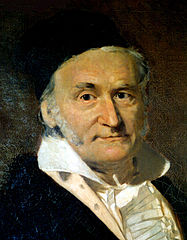
\includegraphics{Carl_Friedrich_Gauss.jpg}
\\

\begin{math}
    A= \left[
    \begin{array}{ccc}
        1 & 0 & 2\\
        4 & 3 & 5\\
        1 & 0 & 1
    \end{array}
    \right]
    \qquad
\end{math}


\newpage
\begin{thebibliography}{2}
%\begin{enumerate}
\bibitem{1} internet 
\url: $http://pl.wikipedia.org/wiki/Macierz_odwrotna$
\bibitem{2} J. Topp: Algebra liniowa
%\end{enumerate}
\end{thebibliography}


\end{document}
